\chapter*{Organisation du projet}
\addcontentsline{toc}{chapter}{Organisation du projet}
\markboth{Organisation du projet}{Organisation du projet}
\label{sec:organisation}


\section*{Work Breakdown Structure}
\addcontentsline{toc}{section}{Work Breakdown Structure}
Le WBS suivant présente les principales tâches à effectuer pour notre projet.

\begin{figure}[!h]
	\centering
	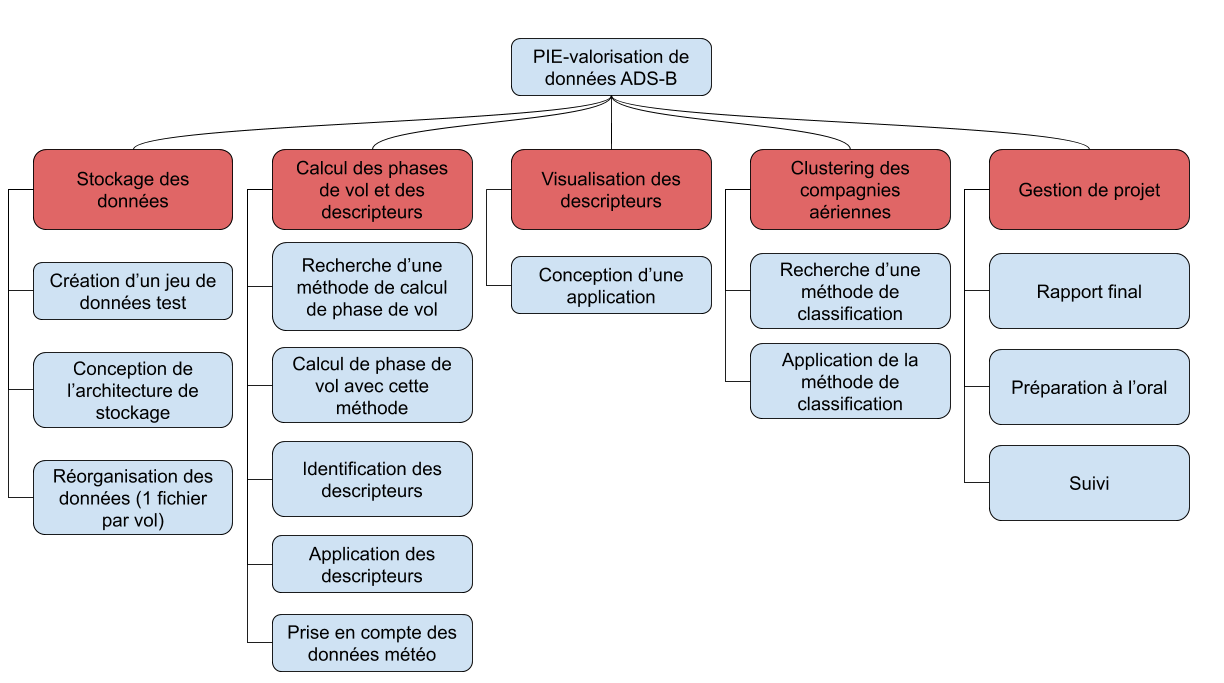
\includegraphics[width=12cm]{WBS}
	\caption{WBS}
	\label{fig:wbs}
\end{figure}



\section*{Planning}
\addcontentsline{toc}{section}{Planning}
Les figures \ref{fig:mvp-plan}, \ref{fig:gestion-proj} et \ref{fig:r1-plan} montrent le planning que nous allons suivre pour réaliser notre projet.

\begin{figure}[!ht]
	\centering
	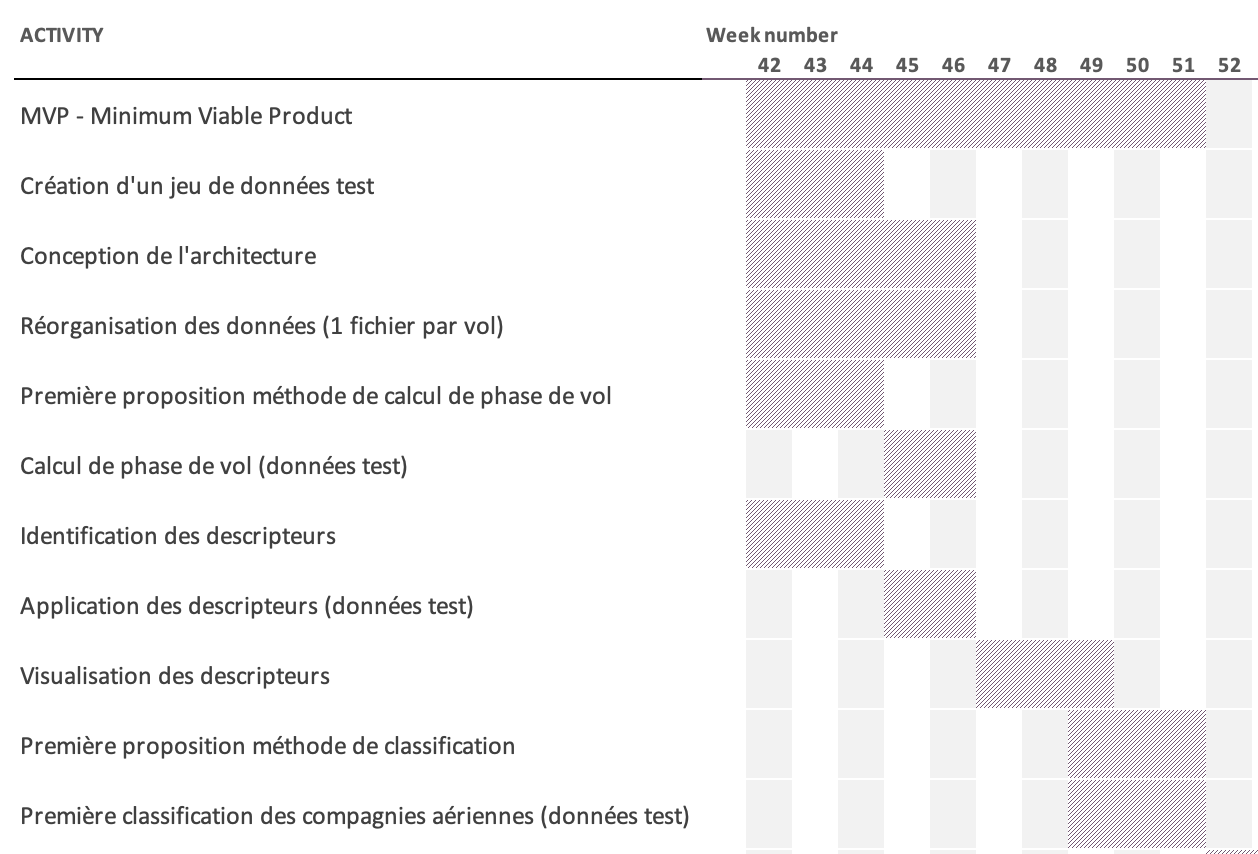
\includegraphics[width=15cm]{MVP planning}
	\caption{planning associé au produit minimal(MVP)}
	\label{fig:mvp-plan}
\end{figure}

\begin{figure}[!ht]
	\centering
	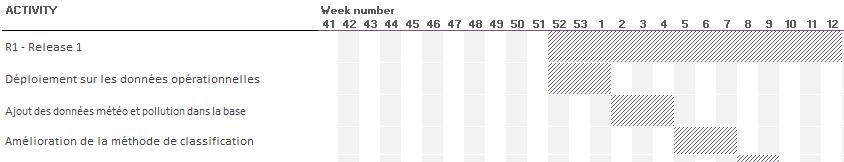
\includegraphics[width=15cm]{R1 planning}
	\caption{planning associé au produit final}
	\label{fig:r1-plan}
\end{figure}

\begin{figure}[!ht]
	\centering
	\includegraphics[width=15cm]{gestion projet}
	\caption{planning associé à la gestion de projet}
	\label{fig:gestion-proj}
\end{figure}

\section*{Association des taches aux membres du projet}
\addcontentsline{toc}{section}{Association des taches aux membres du projet}
La matrice en figure \ref{fig:raci} présente l'attribution des tâches à chaque membre du projet:


\begin{figure}[!h]
	\centering
	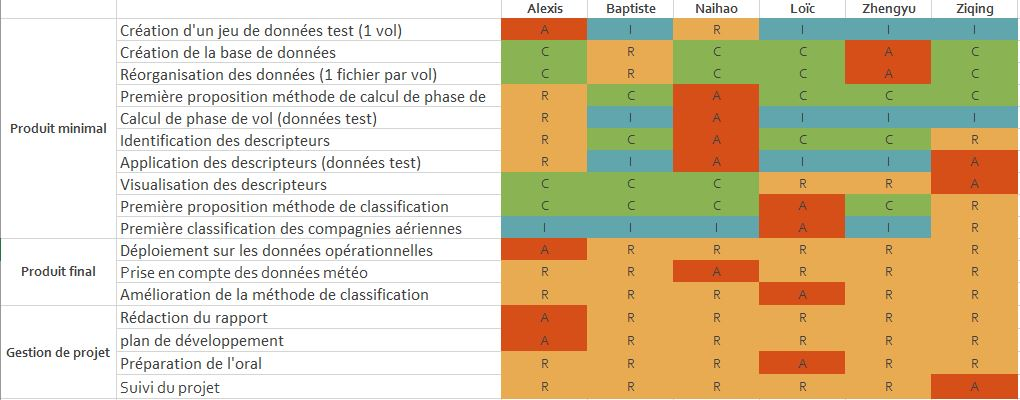
\includegraphics[width=15cm]{RACI}
	\caption{matrice RACI, R:responsible, A:accountable, C:consulted, I:informed}
	\label{fig:raci}
\end{figure}
\section*{Suivi}
\addcontentsline{toc}{section}{Suivi}
Afin que la communication au sein du projet soit de bonne qualité, nous avons mis en place un drive google où sont stockés les documents qui concernent la gestion du projet (cahier charge, compte rendu de réunion,...). Afin d'assurer les travaux de développement et de rédaction de document qui sont souvent fait en équipe, nous avons mis en place un répertoire github. Ces deux répertoires sont accessibles et modifiables depuis n'importe quel poste et par n'importe quel membre du projet. 

Chaque semaine, une réunion sera organisé ce qui permettra de faire un point régulier de l'avancement du projet. Il permettra aussi à chaque membre de poursuivre les tâches qui lui sont attribuées.

D'autre part, nous utiliserons la librairie pandas sous python pour assurer le traitement des données, ainsi que django pour réaliser des applications web. En ce qui concerne la partie gestion de projet, nous utiliserons la suite office ainsi que latex pour rédiger les rendus.

\section*{Organigramme}
\addcontentsline{toc}{section}{Organigramme}
Voici ici l'organigramme correspondant à notre projet.
\begin{figure}[!ht]
	\centering
	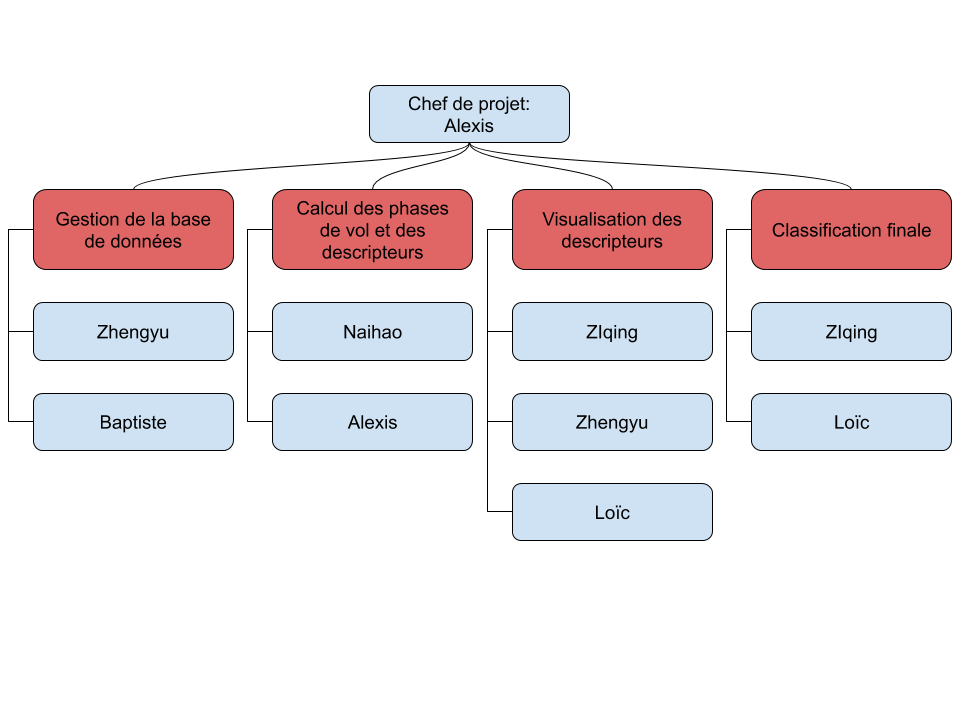
\includegraphics[width=10cm]{Organigramme}
	\caption{Organigramme}
	\label{fig:Organigramme}
\end{figure}



\section*{Gestion des risques et Opportunités}
\addcontentsline{toc}{section}{Gestion des risques}
La gestion des risques est un point clé dans le succès du projet car elle permet d'agir de manière à ce que les risques identifiés arrivent avec la probabilité la plus faible possible. En concertation avec les membres du projet, nous avons identifié les risques suivant:

\begin{itemize}
	\item Perte des données. Une panne matériel peut survenir à tout moment et endommager les données. Ce risque reste assez faible et on peut toujours récupérer les données en les téléchargeant une nouvelle fois.
	
	\item Difficulté d'accès aux données. Si les données sont stockées sur un ordinateur personnel, il y a un risque que cela ralentisse le développement des codes de calculs. C'est pourquoi nous avons envisagé de stocker les données sur un disque accessible depuis n'importe quel ordinateur de l'école.
	
	\item Logiciel inconnu par certain membre du groupe. Nous devrons prendre en compte le fait que tous les membres ne connaissent pas les librairies utilisés et donc évaluer le temps de travail en fonction de cela.
	
	\item Crise du coronavirus. Dans le contexte actuel, il est très probable qu'un des membres tombent malade ou que la communication entre les membres soient plus difficile. Nous devons donc faire en sorte que la majorité des tâches puissent se faire depuis un ordinateur personnel.
	
	\item Mauvaise communication interne. La plupart du travail sera faite en dehors des créneaux prévus pour le PIE. Une mauvaise communication pouvant entrainer un retard dans l'exécution du projet, nous allons mettre en place un groupe de conversation messenger ainsi qu'un drive Google où seront déposés les documents relatifs à la gestion du projet.
	
\end{itemize}


Nous avons listé ci-dessous des opportunités qui peuvent nous permettre d'améliorer le développement du projet.
\begin{itemize}
	\item Matériel informatique de l'école. L'école dispose de ressource informatique importante qui peuvent nous permettre d'effectuer des calculs rapidement et de stocker une quantité importante de données. Afin de profiter de cela, nous avons fait une demande de matériel à l'école.
	\item La librairie Openap permet de calculer les différentes phases d'un vol. En parvenant à l'utiliser, on peut gagner beaucoup sur cette tâche du projet. Elle est de plus très bien documentée, son utilisation sera donc probablement assez simple.
\end{itemize}
%%% Local Variables: 
%%% mode: latex
%%% TeX-master: "isae-report-template"
%%% End: 